
\chapter{Implementation}\label{avs:implementation}

\section{Tools}

The programming language chosen to implemented the system was C++.
The arguments leading to this choice was:
\begin{itemize}
\item Most of the group members had some earlier experience with the language.
\item It allows for a high level of abstraction without losing control of the
underlying hardware.
\item The code can be easily parallellized for shared memory machines using OpenMP.
\item Many libraries exist for C++ that implement highly optimized linear algebra
functionality.
\end{itemize}
Other languages considered were Matlab and C.
The tools chosen to visualize the resulting data are gnuplot and mencoder. Writing a
program using OpenGL was considered, but dismissed on the grounds of being too time consuming.

\section{Program design}

\begin{figure}[!h]
  \begin{center}
    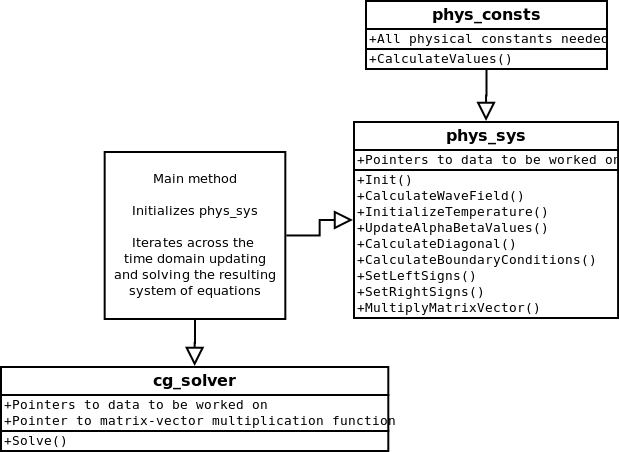
\includegraphics[width=0.5\linewidth]{classdiagram.png}
  \end{center}
  \caption{Class diagram of c++ implementation}
  \label{fig:classdiagram}
\end{figure}
The program mainly consist of three parts:
\begin{itemize}
\item C++ implementation of matrix representations of the discretized equations.
\item C++ implementation of the conjugate gradient method for solving the
equations described.
\item Bash script for generating plots and and movie of the generated data.
\end{itemize}
See \cref{fig:classdiagram} for a class diagram of the C++ implementation.
The Bash script is not discussed in further detail as it is considered to be
very simple. See \cref{ap:source_code} for source code and scripts.

\section{The physical system}

The main task of the physical system is to implement a matrix-vector multiplication
procedure for the heat equation to be used in the conjugate gradient method, 
a method for calculating the heating properties of the microwave, and a method 
for calculating the velocity of mass transfer.

\subsection{Partitioning of the problem}

The problem is to perform the multiplication of a sparse, symmetric matrix with a
vector. To describe this procedure we have vectors $a$, $b$ and $t$ containing alpha,
beta, and temperature values respectively. The alpha values represent the heat 
conduction properties, the beta values describe the substance's ability to be heated
by microwaves and the temperature values naturally contains the temperatures. We need
these vectors because each point in the grid contains a particular substance in
a particular phase.
\begin{figure}[!h]
  \begin{center}
    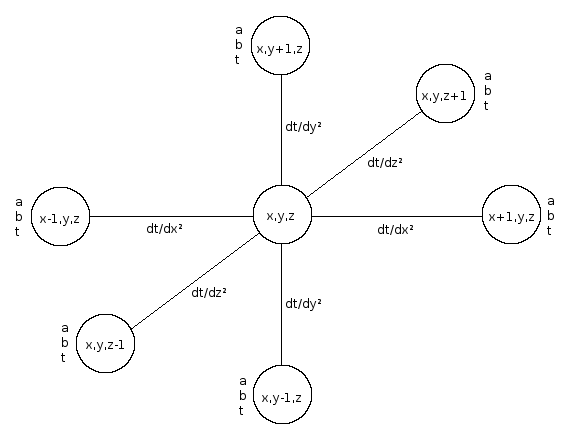
\includegraphics[width=0.5\linewidth]{stencil.png}
  \end{center}
  \caption{Stencil}
  \label{fig:stencil}
\end{figure}
\begin{figure}[!h]
  \begin{center}
    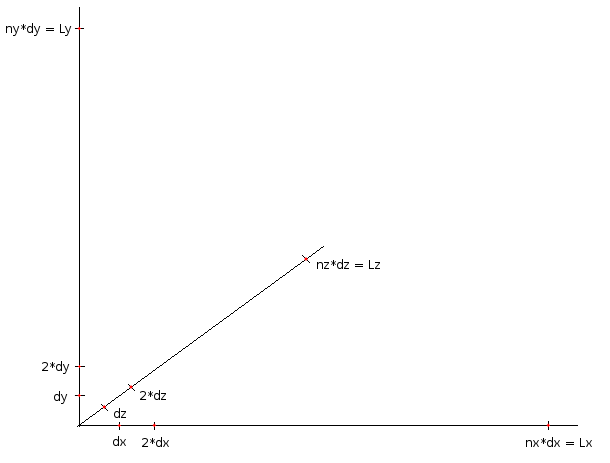
\includegraphics[width=0.5\linewidth]{grid.png}
  \end{center}
  \caption{Grid}
  \label{fig:grid}
\end{figure}
We say that position $j$ of the vectors is given by:
\begin{equation}
j = z\cdot n_x\cdot n_y + y\cdot n_x + x
\end{equation}
where $n_x$, $n_y$, $n_z$ is the number of points in the $x$, $y$ and $z$ directions
respectively, and $x$, $y$ and $z$ is the points on the grid, See \cref{fig:grid} and
\cref{fig:stencil} \\

The center of the stencil, given by $j$, can be described by the equations:
\begin{eqnarray}
  x & \cong & j\%n_x \\
  y & \cong & (j/n_x)\%n_y \\
  z & \cong & j/n_x/n_y 
\end{eqnarray}
where $/$ and $ \% $ is the integer division and modulo operators respectively.
In addition to this, we define two more vectors and one more matrix:

The offset matrix represents the neighbours in the stencil (see \cref{fig:stencil}):
\begin{equation}
O =
\left[
\begin{array}{ccc}
0 & 0 & -1 \\
0 & -1 & 0 \\
-1 & 0 & 0 \\
0 & 0 & 0 \\
1 & 0 & 0 \\
0 & 1 & 0 \\
0 & 0 & 1 \\
\end{array}
\right]
\end{equation}

The delta vector representing the difference in time and distance used in the heat
equation:
\begin{equation}
D = \{ \frac{dt}{dz^2}, \frac{dt}{dy^2}, \frac{dt}{dx^2}, 0, \frac{dt}{dx^2}, \frac{dt}{dy^2}, \frac{dt}{dz^2} \}
\end{equation}

The vector containing the offsets relative to the diagonal in the matrix we are multiplying
with:
\begin{equation}
R = \{ -n_x\cdot n_y, -n_x, -1, 0, 1, n_x, n_x\cdot ny \}
\end{equation}

Note that the indexing of these vectors and matrices correspond, so by looping through them,
We have all the information we need to perform the necessary operations.

\subsection{Updating alpha and beta values}

When updating the alpha and beta values, we simply loop through the temperature
vector, and update the alpha and beta vectors to their correct values using the
physical constants describing the substance at that point.

\subsection{Calculating the distribution of the microwave effect}

This is done according to \cref{eq:effektfordeling} and by multiplying the
resulting distribution by the microwave effect and dividing by the volume at each point
in the grid.

\subsection{The matrix-vector multiplication procedure}

The matrix-vector multiplication procedure takes advantage of the fact that our 
matrix is sparse and that our problem is well defined. Thus the algorithm used
will complete in $m$ iterations where $m$ is the number of non-zero entries in 
the matrix. $m$ is approximately equal to $7\cdot n$.

\section{The conjugate gradient method as an iterative algorithm}

The method (conjugate gradient) used to solve the system of equations is based on 
the steepest descent algorithm, however, it results in the exact solution within
$n$ iterations. This is, however, assuming we have infinite floating point
accuracy. \\

The iterative conjugate gradient method lets us define an acceptable error, and stops
once our solution has an error within what is acceptable.
In our implementation, we recompute the correct residual to avoid accumulation of
floating point precision errors. But this is not done at each iteration, and may
result in the need of more than $n$ iterations for the algorithm to complete.

\section{The main procedure}

\begin{itemize}
  \item Initialize problem; define grid-size, dimensions of bacon, partitioning of fat vs meat
  and internal and external temperature.
  \item Allocate necessary memory
  \item Initialize physical system
  \item Initialize internal temperature
  \item Calculate boundary conditions
  \item Calculate microwave field
  \item Initialize conjugate gradient solver
  \item loop
  \begin{itemize}
    \item Update alpha and beta values
    \item Calculate diagonal
    \item Set signs for right side multiplication (t=n)
    \item Multiply right side of heat equation
    \item Add microwave effect to right side of equation
    \item Set signs for left side of equation (t=n+1)
    \item Solve using conjugate gradient method
    \item Save data to file every N iterations
  \end{itemize}
\item Deallocate memory
\end{itemize}

\section{Parallel speedup}

The program was tested with $n_x=n_y=n_z=15$ giving $n=n_x\cdot n_y\cdot n_z=3375$ and $n_t=100000$.
The sequential version of the program ran in 342 seconds. 
The parallell version ran in 194 seconds (2 cores) and 181 seconds (4 cores).
This gives us a speedup of:
\begin{equation}
S_p(2) = \frac{T_s}{T_{p,2}} = \frac{342}{194} = 1.76
\end{equation}
and 
\begin{equation}
S_p(4) = \frac{T_s}{T_{p,4}} = \frac{342}{181} = 1.89
\end{equation}

The reason the speedup between 2 and 4 cores was so small may be due to a lack of
parallelizable work. The code can only be parallelized on the spatial work ($n$) of the
heat equation, and not across the time domain ($n_t$). Thus most of the work involved in
this program is sequential. \\

The conjugate gradient method is not parallellizable either (except for the linear algebra functions it
uses). Thus, the total of parallelizable work is just $n$, which for this example may be too small.

\section{Resulting plots}
Three resulting plots are displayed here, please also refer to the animation
movie file attached. These plots were made with a single bacon slice of
dimensions 15cm x 5cm x 0.1 cm modelled in a 750 W microwave oven. The
simulation was run without a stop criterion for 120 seconds, ensuring that the
interesting time interval is at least covered by the simulation. \\

\begin{figure}[!h]
  \begin{center}
    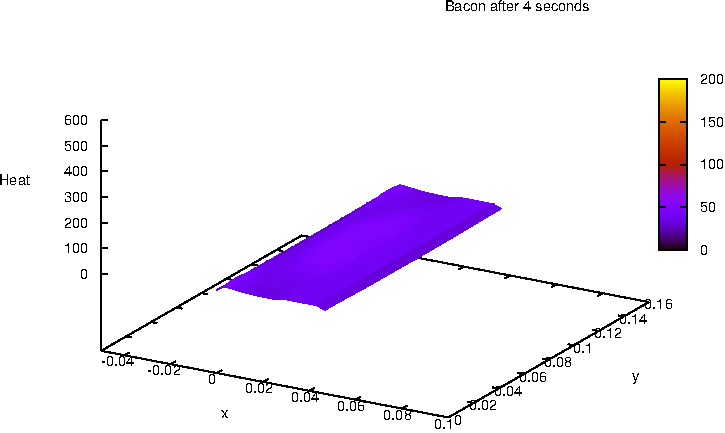
\includegraphics[width=0.75\textwidth]{bacon-4sec.pdf}
  \end{center}
  \caption{A slice of bacon after four seconds in a microwave oven}
  \label{fig:bacon-4sec}
\end{figure}

The first plot, \cref{fig:bacon-4sec}, shows bacon after four seconds in the microwave oven. As
expected, not much is happening, but it is noted that the temperature is higher
in the left part of the bacon strip, corresponding to the fat, in accordance
with theoretical expectations.\\

\begin{figure}[!h]
  \begin{center}
    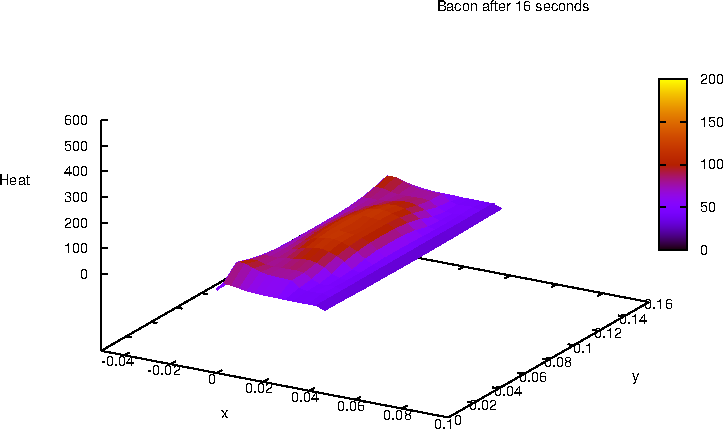
\includegraphics[width=0.75\textwidth]{bacon-16sec.pdf}
  \end{center}
  \caption{A slice of bacon after sixteen seconds in a microwave oven}
  \label{fig:bacon-16sec}
\end{figure}

The second plot, \cref{fig:bacon-16sec}, is taken at 16 seconds. Here stuff is
starting to happen, and it is interesting to note that the temperature in the
left part of the bacon strip is the highest here, the opposite of the situation
at 4 seconds. This is because the fat has started melting, and the melting
process makes the heating process slow down, again in accordance with
theoretical expectations. \\

\begin{figure}[!h]
  \begin{center}
    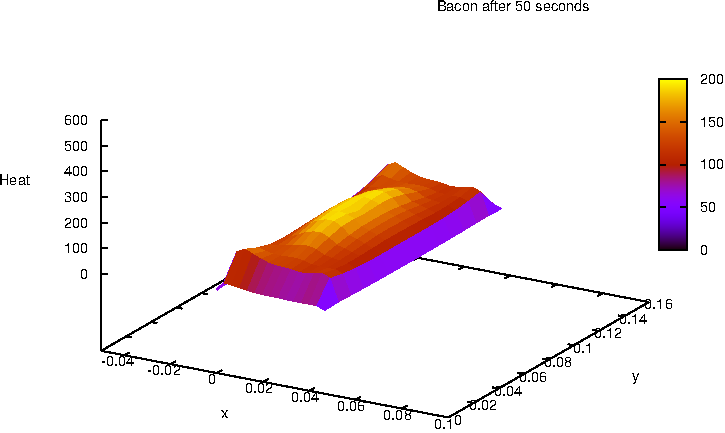
\includegraphics[width=0.75\textwidth]{bacon-50sec.pdf}
  \end{center}
  \caption{A slice of bacon after fifty seconds in a microwave oven}
  \label{fig:bacon-50sec}
\end{figure}

The third plot, \cref{fig:bacon-50sec}, is taken at 50 seconds. This is finished
bacon, with meat temperatures well above the Maillard critical temperature. The
fat temperature has almost caught up with the meat, and the bacon should be very
tasty at this point.


\section{Unimplemented functionality}

Due to time constraints and unforeseen complications, the transport equation was not implemented, 
however a significant amount of effort was put into the implementation before it was 
abandoned. The numerical schemes implemented in an attempt at solving the
equation were:

\begin{itemize}
  \item Forward Euler
  \item Runge-Kutta
\end{itemize} 

Forward Euler was dismissed as the time steps had to be too small to be practical.
The Runge Kutta method also gave us some strange and unforeseen results, as the term in 
the equation that was supposed to keep the velocity field equal to $0$ until the substances
started melting, caused the velocity field to blow up to infinity. Other issues was that
the nodes close to the boundary, seems to never reach melting point
temperatures.\\

After looking closely at the differential equations and their discrete equivelents, a number
of practical issues surfaced that would require modifications to existing code
as well, so the continued development of the transport equation was dismissed
as the project was close to its end.\\

Further work on the mass-transfer equations would involve time-dependant boundary conditions,
crank-nicholson discretization, and solving them with the conjugate gradient method.

Since the mass transfer equation was not properly implemented, the stop criteria was not 
implemented either, as it turned out to be more practical to just run the simulation for as 
many seconds as needed, say 120, and inspect the resulting plots to find an
optimal cooking time of about 50 seconds.
